\section{Orthogonality}
\subsection{Orthogonal vectors and subspaces}
\textbf{Orthogonal vectors:} $x$ and $y$ are orthogonal iff $x^Ty = 0$.\\
\textbf{Length of a vector:} $\|x\| = x^Tx$.\\
\textbf{Orthogonal subspaces:} Two subspaces $V$ and $W$ are said to be 
orthogonal if $\forall v \in V$ and $\forall w \in W$ $v \perp w$.\\
\textbf{Orthogonal complement:} Given a subspace $V$ in $\mathbb{R}^n$, the 
space of all vectors orthogonal to $V$ is called orthogonal complement of $V$.
It is denoted by $V^{\perp}$.


\begin{mdframed}[backgroundcolor=SlateGray2!40,linecolor=Firebrick4]
\textbf{Theorems:}
\begin{itemize}
\item If a set of vectors $v_1, v_2, \cdots, v_k$ of non-zero length are 
        mutually perpendicular, then those vectors are linearly independent.
\item Row space is orthogonal complement of null space.
\item Column space is orthogona complement of left null space. 
\end{itemize}
\end{mdframed}


\subsubsection{A deeper meaning of matrix multiplication}
The matrix multiplication $Ax$ transforms the rowspace componenet of $x$ ($x_r$) to column-space of A and the nullspace component of $x$ ($x_n$) to $0$.\\
Here $x = x_r + x_n$.\\
\textit{The real action is between rowspace and column space.}



\subsection{Cosines and Projections onto lines}

\textbf{Cosine} The cosine of the angle between any two non-zero vectors is defined as follows:
$$cos\theta = \frac{a^Tb}{\|a\|\|b\|}$$

\textbf{Law of cosines}
$$\|b - a\|^2 = \|a\|^2 + \|b\|^2 - 2\|a\|\|b\|cos\theta$$

\textbf{Schwarz inequality}
$$\|a^Tb\| \leq \|a\|\|b\|, \because cos\theta \leq 1$$\\

\subsubsection{Projection onto a line (1D subspace)}

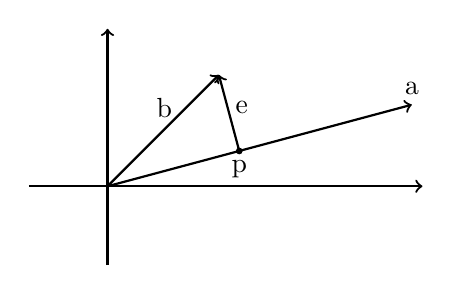
\begin{tikzpicture}
	\draw[thick, ->] (-1,0) -- (0:4);
	\draw[thick, ->] (0,-1) -- (90:2);
	\draw[thick, ->] (0,0) -- (15:4);
	\draw[thick, ->] (0,0) -- (45:2);
	\draw[thick, ->] (15:1.732) -- (45:2);
	\filldraw[black] (15:1.732) circle (1pt) node[anchor = north] {p};
	\node[anchor = west] at (1.50244, 1.000) {e};
	\node[anchor = west] at (0.5,1) {b};
	\node[anchor = south] at (15:4) {a};
\end{tikzpicture}

$p$ is projection of $b$ on $a$. $\therefore p = xa $ for some x.\\

$$e = b - p \text{ and } e \perp  a,$$
$$\therefore a^T(b-xa) = 0$$
$$xa^Ta = a^Tb$$
$$\implies x = \frac{a^Tb}{a^Ta}$$
\begin{center}
\framebox{$p = a\frac{a^Tb}{a^Ta}$}
\end{center}

This can be written as,\\
$p = \frac{aa^T}{a^Ta}b = Pb$, where $P = \frac{aa^T}{a^Ta}$ is the projection matrix of $a$.
	

\textbf{Properties of P}\\
\begin{itemize}
	\item $C(P)$ = line through $a$.
	\item Rank(P) = 1.
	\item $P$ is symmetric: $P = P^T$
	\item $P^2=P$
\end{itemize}

\subsubsection{Projection onto a higher dimension subspace}

\textbf{Finding projection of } $b$ \textbf{on} $A$\\
Let $p$ be the projection of $b$ on subspace spanned by columns of $A$, 
then there exists $\hat{x}$ such that $A\hat{x} = p$\\
$b - p \perp A \implies A^T(b-A\hat{x}) = 0$ \\
$\therefore \hat{x} = (A^TA)^{-1}A^Tb$\\
$\therefore p = A(A^TA)^{-1}A^Tb$\\
Here the projection matrix $P = A(A^TA)^{-1}A^T$\\
If $A$ is invertible then $P = I$ 

\begin{mdframed}[backgroundcolor=gray!20]
$A^TA$ has the same nullspace of $A$\\
i.e., $A^TA$ is invertible if columns of $A$ are independent.
\end{mdframed}

\vspace{12pt}

\textbf{Least squares problem}
Solve: $Ax =b$\\
\begin{itemize}
\item Normal equations: $A^TA\hat{x} = A^Tb$\\
\item Best estimate: $\hat{x} = (A^TA)^{-1}A^Tb$\\
\item Projection: $p = A\hat{x} = A(A^TA)^{-1}A^Tb$\\
\item $b = p + e$\\
\item $p$ is in $C(A)$\\
\item $e$ is in N$(A^T)$\\
\item If $b$ is in C(A), $p = A(A^TA)^{-1}A^Tb = A(A^TA)^{-1}A^TAx = Ax = b$
\item If $b$ is in $N(A^T)$, $p = A(A^TA)^{-1}A^Tb = A(A^TA)^{-1}0 = 0$
\item If $A$ is invertible, $p = A(A^TA)^{-1}A^Tb = b$
\item (I think) $\|e\|^2 = \|b-p\|^2$ is the squared error.

\end{itemize}


\subsection{Orthogonal basis and Gram-Schmidt}

\textbf{Orthogonal basis:}
A set of bases, $q_1, q_2, \cdots, q_k$, is said to be orthogonal bases, 
if for all $i \neq j$ $q_iTq_j = 0$.

\textbf{Orthonormal basis:} Orthonormal bases,$q_1, q_2, \cdots, q_k$, satisfies the following property:\\

% \begin{equation}
$$
	q_i^Tq_j = 
	\begin{cases}
		1 \text{ if } i = j.\\
		0 \text{ otherwise} \end{cases}	
$$
% \end{equation}

\subsubsection{Gram-Schmidt process}
\begin{itemize}
	

\item Eg: A case with two bases $a$ and $b$:\\
$a' = a$\\
$b'= b - \frac{aa^T}{a^Ta}b$, here, $b'= e$ and $b = p + e$\\

\item Eg: Case with three bases $a, b$ and $c$.\\

$a' = a$\\
$b' = b - \frac{aa^T}{a^Ta}b$\\
$c' = c - \frac{aa^T}{a^Ta}c - \frac{bb^T}{b^Tb}c$\\
From $c$ subtract projection of $c$ on $a$ and projection of $c$ on $b$.

\end{itemize}
